\documentclass{article}
\usepackage[latin1]{inputenc}
\usepackage[pdftex]{color}
\usepackage[pdftex]{graphicx}
\usepackage[T1]{fontenc}
\usepackage{amsfonts}
\usepackage{amsmath}
\usepackage{cancel}
\usepackage{array}
\usepackage{xspace}
\usepackage{verbatim}
\usepackage{mathabx}
\usepackage{longtable}
\setlength{\parindent}{0pt}

\title{GenAMap Data Importing}
\author{}
\date{}

\begin{document}

\maketitle

\begin{raggedright}
\hyphenpenalty=10000
\exhyphenpenalty=10000
For further questions / comments / suggestions, please contact genamapsupport@cs.cmu.edu

\end{raggedright}

\section{Introduction}

Below, we describe how data should be formatted for importing into GenAMap. We suggest that you read the instructions carefully to avoid import errors and algorithm failures. Note that GenAMap is a software under development. Hence, some of the conventions below may seem unnecessary complex. We are working on improving the importing mechanisms and in the meantime, kindly ask for your patience. \\

Also, whenever GenAMap provides multiple formatting options for importing a certain type of data, please only use the option that is described below, as the others might not yet have been thoroughly tested. 

\section{Importing Marker Data}

\paragraph{Overview} Marker Data has three components: The actual marker (=SNP) values, labels for each sample / individual, and labels for each marker. The marker values take the form of an $N$ by $d$ matrix where $N$ is the number of samples and $d$ is the number of markers. Each row corresponds to a sample, each column corresponds to a marker and each entry represents the value of the marker corresponding to the column of the entry for the sample corresponding to the row of the entry. A sample label is a simple string. A marker label has three components: A marker name, the number of the chromosome the marker is on and the location of the marker along that chromosome (in base pairs).

\paragraph{How to format the data} Please provide the data as three files: a marker value file, a sample label file and a marker label file. The marker value file should be an $N$ by $d$ matrix (as described above) in a tab-delimited format. It should only contain numerical values. The sample labels should be in a file with $N$ lines, where each line is the label for a particular sample. These can be arbitrary but have to be unique. The marker labels should be arranged as a $d$ by 3 tab-delimited matrix, where each line contains the chromosome number, the marker name and the marker location in that order. The marker names can be arbitrary and the chromosome number and marker location must be integers. It is possible to provide dummy values for chromosome number and marker location, but note that no pair of (chromosome number, marker location) may appear twice. Also, marker names must be unique. While the values of $N$ and $d$ that define the sizes of these files can be arbitrary, they have to be consistent between the three files.\\

Marker Data can be used to run association algorithms and other algorithms. Note that while it is permitted for marker values to take any numerical form, including floating-point values, a few algorithms (currently PLINK, Structure and PopAnal) incorporated in GenAMap do not work unless the marker value matrix only contains values 0,1 and 2. The chromosome number and marker location are used in the chromosome browser and to the define the x-axis in the Manhattan plot. If the chromosome number and marker location are not available, you can use dummy values inside the marker label file as shown in `markerKeysDummy.txt'. The marker name is used to link to dbSNP and SGD (Saccharomyces Genome Database). In order to interact successfully with these external databases through GenAMap, the marker name must be an rs\# (for dbSNP) or the name of the gene the marker is on (for SGD). The sample labels have no special purpose.

\paragraph{How to import the data} Bring up the marker import dialog as shown in Figure 1. Choose the project to add the data to and the name of the Marker Data set itself. Provide the paths to the three input files, then click ``import''.

\paragraph{Example data files} We provide 4 files: markerVals.txt, markerLabelsDummy.txt, markerLabelsYeast.txt and sampleKeys.txt. These can be used directly for importing. We have provided two different marker label files. markerLabelsDummy.txt contains dummy values for marker name, chromosome number and marker location. If these values are not available for your data set, it is suggested that you create a marker label file in that form. markerLabelsReal.txt illustrates what marker labels from a real dataset might look like. You can use these marker name to access he SGD database. Note that the actual marker values (as well as all other numerical data) provided for the purposes of this tutorial is synthetic and any resemblance to real data is coincidental.

\section{Importing Trait Data}

\paragraph{Overview} Trait data in GenAMap can stand for gene expression data or phenotype data. Similar to Marker Data, Trait Data has three components: The actual trait values, labels for each sample / individual and labels for each trait. The trait values take the form of a $N$ by $t$ matrix where $N$ is the number of samples and $t$ is the number of traits. Each row corresponds to a sample, each column corresponds to a trait and each entry represents the value of the trait corresponding to the column of the entry for the sample corresponding to the row of the entry. Sample labels and trait labels are both simple strings.

\paragraph{How to format the data} Please provide the data as three files: a trait value file, a sample label file and a trait label file. The trait value file should be an $N$ by $t$ matrix (as described above) in a tab-delimited format. This file should only contain numerical values. The sample labels and trait labels should each be in a file with $N$ / $t$ lines respectively, where each line is the label for a particular sample / trait. These can be arbitrary but have to be unique. \\

Trait Data can be used to run association algorithms, network algorithms, and other algorithms. Trait values can take any floating-point value. Trait labels are used to link to external resources Google and UniProt, with the latter only applicable if traits are gene expressions. To use these facilities, trait labels must be interpretable by the external databases. For gene expression traits, trait labels are also used to perform GO analysis. For this, trait labels must take the form of gene names. To see which gene naming conventions GenAMap supports for a particular species, navigate to the folder `goSpecies' and open the file for the species you are interested in. The trait labels should appear in this table to facilitate GO analysis. Sample labels have no particular purpose. Note that if different Trait Data sets / Marker Data sets are to be used within the same algorithm, the sample label files provided for them must contains the same samples. The rows in the value files are then matched accordingly.

\paragraph{How to import the data} Bring up the trait import dialog as shown in Figure 2. Choose the project to add the data to and the name of the Trait Data set itself. Click on the radio button `no row or column headers'. Provide the paths to the three input files. In order to use GO analysis in GenAMap, you must provide the name of the species the data is about, then click `import'.

\paragraph{Example data files} We provide 5 files: traitVals.txt, traitLabels.txt, geneVals.txt, geneLables.txt and sampleLabels.txt. These can be used directly for importing. You can either use the first, second and fifth file or the third, fourth and fifth file together. traitLabels.txt contains dummy values as trait labels. If your dataset does not contain trait labels, it is suggested you generate a file of a similar form. geneLabels.txt contains actual gene names as labels.

\section{Importing other data}

\subsection{Network Data}

Networks are edge-weight matrices of graphs over traits. Hence, they take the form of a square, symmetric, real-valued matrix. The data should be a provided as a tab-delimited matrix of size $t$ by $t$, where $t$ is the number of traits in the corresponding Trait Data set. Please make sure that the columns / rows of the matrix align with the columns of the Trait Data set for which the Network is provided. To import the data, bring up the import dialog as in Figure 3. Choose the project to add the data to, the Trait Data set the Network is for, and the name of the Network itself. Click the radio buttons `Load from File' and 'Tab delimited format', provide the path to the file and click `import'. The example Network files are `traitNetwork.txt' and `geneNetwork.txt'. These are the ground truth Networks for the provided Trait Data sets.

\subsection{Association Data}

Association Data sets describe the association strengths between markers and traits. They take the form of a $d$ by $t$ matrix, where $d$ is the number of markers and $t$ is the number of traits. The $i,j$'th entry is the association strength between marker $i$ and trait $j$. The data should be provided as a tab-delimited matrix. When an Association Data set it imported, it must reference a Marker Data set and a Trait Data set. In order to be able to use all functionalities in GenAMap, please make sure the markers (=rows) align with the markers in the referenced Marker Data set and the traits (=columns) align with the traits in the referenced Trait Data set. To import the data, bring up the import dialog as in Figure 4. Choose the project to add the data to, the name of the Marker Data set and Trait Data sets the Association Data set is for, and the name of the Association Data set itself. Click the radio button `Load from File', provide the path to the file and click `import'. The example Association Data files are `traitAssociations.txt' and `geneAssociations.txt'. These are the ground truth Associations between the provided Marker Data set and the two provided Trait Data sets.

\subsection{Clustering}

A Clustering is a re-ordering / permutation of traits that pulls related traits close together. It always references a Trait Data set. This data should be imported as a single file where each row is an integer corresponding to the index of the trait (= the column index in the trait matrix), and each such index appears exactly once. To import the data, bring up the import dialog as in Figure 5. Choose the project to add the data to, the name of the Trait Data set the Clustering is for, and the name of the Clustering itself. Click the radio button `Load from File', provide the path to the file and click `import'. The example file is `traitClustering.txt'. It is the ``ground truth Clustering'' for `traitVals.txt'. If you import `traitNetwork.txt' and `traitClustering.txt' and apply the latter to the former in GenAMap, the visualization will expose the structure in the data.

\subsection{Subset}

A Subset is a list of trait labels that can be used to direct GenAMap's visualization tools to places of interest, for example by enabling the user to view all traits with a certain used-defined property in a JUNG view. It should be provided as a file where each line contains a single trait label. The subset will then simply be the set of traits with those labels. To import the data, bring up the import dialog as in Figure 6. Choose the project to add the data to, the name of the Trait Data set the Subset is for and the name of the Subset itself. Click the radio buttons `Load from File' and `Name format', provide the path to the file and click `import'. The example file is `traitSubset.txt'. It contains the most interesting traits in `traitVals.txt'.

\subsection{Feature Data}

Feature Data are a quantitative properties that can be added to all markers in a Marker Data set. Features can, for example, be used to run the Adaptive Multi-Task Lasso. The Feature Data file should be a $d+1$ by $f$ tab-delimited matrix, where $d$ is the number of markers in the Marker Data set and $f$ is the number of features imported. The first row of the matrix indicates the names of the features in string format. The remaining $d$ rows contain the actual feature values, which can be arbitrary real numbers. Please make sure the rows of the Feature Data file align with the columns of the Marker Data set it relates to. Specifically, the marker corresponding to the $i$'th column in the marker value file should be the marker corresponding to the $i+1$'st row in the Feature Data file (remember, the $i+1$'st row is the $i$'th numerical row). To import the data, bring up the import dialog as in Figure 7. Choose the project to add the data to, Marker Data set the Feature Data is for and the name of the Feature Data set itself. Provide the path to the file and click `import'. The example file is `features.txt'.

\subsection{Tree}

A tree is a tree-structure over traits where the direct path between highly related traits tends to be shorter than the direct path between unrelated traits. The traits themselves correspond to the leaf nodes of the tree. To specify the tree data file, you first have to give each node in the tree a name. The leaf nodes must have the same names as the traits as specified in the trait label file. The root node of the tree must have name `Root'. All other nodes can have arbitrary names. The tree data file is specified as an $e$ by 2 tab-delimited matrix, where $e$ is the number of edges in the tree. Each row corresponds to an edge. The first entry in each row should be the name of the child node (the one closer to the leaves) and the second entry should be the name of the parent node (the one closer to the root). Note that the number of edges in the tree is equal to the number of nodes in the tree minus one, as each node has exactly one parent apart form the root. To import the data, bring up the import dialog as in Figure 8. Choose the project to add the data to, the Trait Data set the Tree is for, and the name of the Tree itself. Click the radio buttons `Load from File' and `Parent Child Format', provide the path to the file and click `import'. The example file is `traitTree.txt' and relates to `traitVals.txt'.

\subsection{Population Structure}

A Population Structure in GenAMap is somewhat complicated because that it consist of two different components. Firstly, it contain one or more clusterings of the samples into sub-populations. Secondly, it contains a low-dimensional embedding of the Marker Data set computed via PCA. It is only possible for the user to import a single clustering of the samples. Once the clustering is imported, GenAMap will automatically start an algorithm that performs PCA on the Marker Data set to fill in this missing component of the Population Structure. To specify the clustering, please provide a $d$ by 2 tab-delimited matrix. The first column should contain the sample labels as provided in the sample label file of the Marker Data set (the order is unimportant). The second column should contain the cluster assignment of the samples, as an integer between 1 and $k$, with $k$ the total number of clusters. To import the data, bring up the import dialog as in Figure 9. Choose the project to add the data to, the Marker Data set the Population Structure is for and the name of the Population Structure itself. Click the radio button `Load from FIle', provide the path to the file and click `import'. The example file is `populationStructure.txt'.

\subsection{3-way Association Data and Gene Modules}

At the moment, it is not possible to these types of data. We apologize for this inconvenience. Those features will be available soon.

\clearpage

\begin{figure}
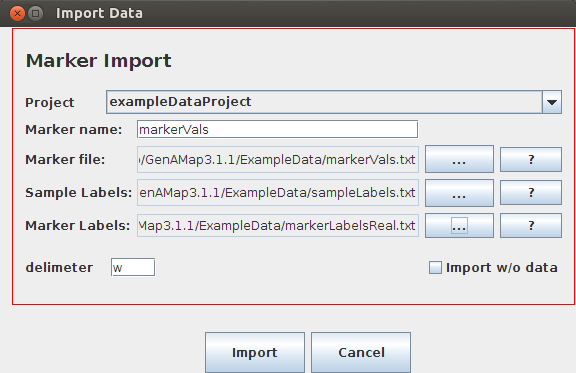
\includegraphics[width=\textwidth]{Figure1.png}
\caption{\textbf{Importing Marker Data}}
\end{figure}

\begin{figure}
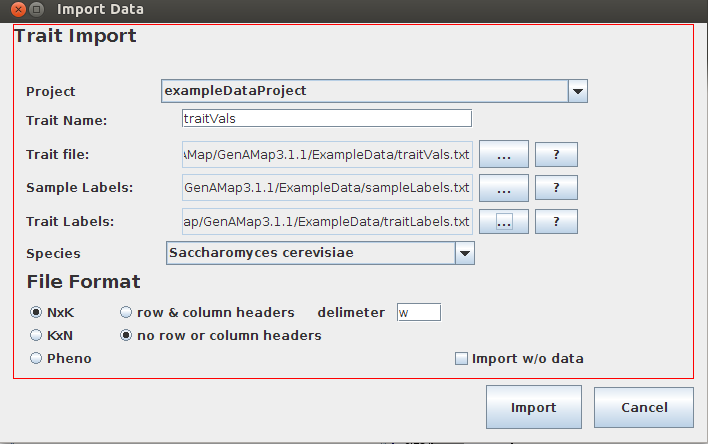
\includegraphics[width=\textwidth]{Figure2.png}
\caption{\textbf{Importing Trait Data}}
\end{figure}

\begin{figure}
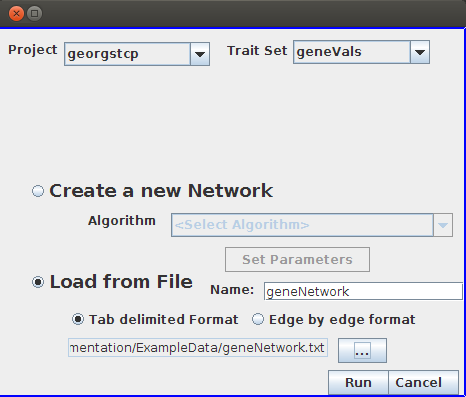
\includegraphics[width=\textwidth]{Figure3.png}
\caption{\textbf{Importing Network Data}}
\end{figure}

\begin{figure}
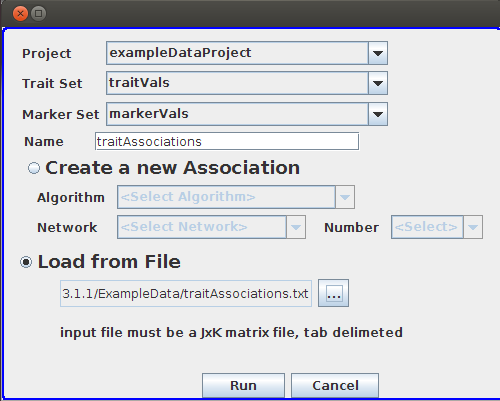
\includegraphics[width=\textwidth]{Figure4.png}
\caption{\textbf{Importing Association Data}}
\end{figure}

\begin{figure}
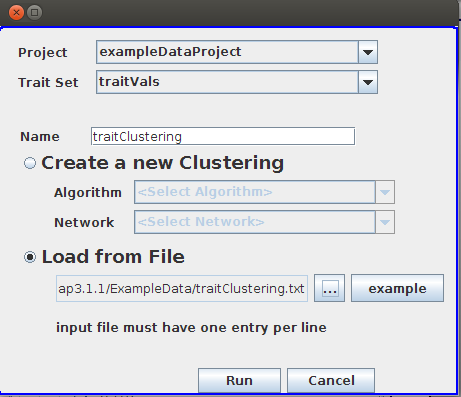
\includegraphics[width=\textwidth]{Figure5.png}
\caption{\textbf{Importing a Clustering}}
\end{figure}

\begin{figure}
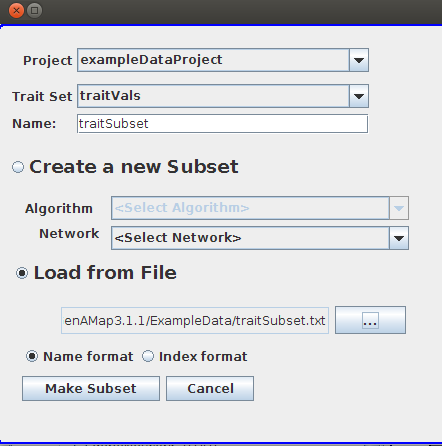
\includegraphics[width=\textwidth]{Figure6.png}
\caption{\textbf{Importing a Subset}}
\end{figure}

\begin{figure}
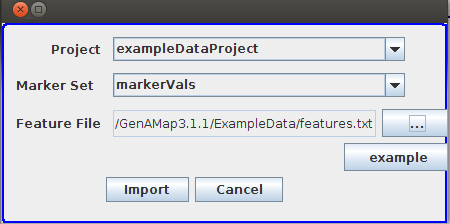
\includegraphics[width=\textwidth]{Figure7.png}
\caption{\textbf{Importing Feature Data}}
\end{figure}

\begin{figure}
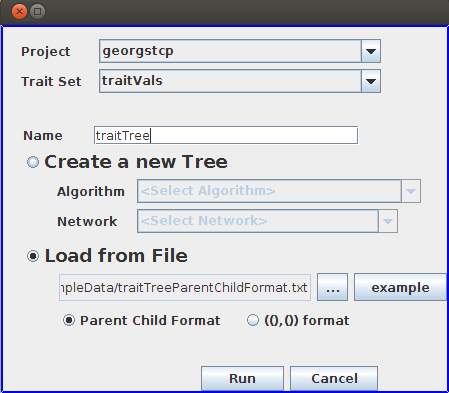
\includegraphics[width=\textwidth]{Figure8.png}
\caption{\textbf{Importing Tree Data}}
\end{figure}

\begin{figure}
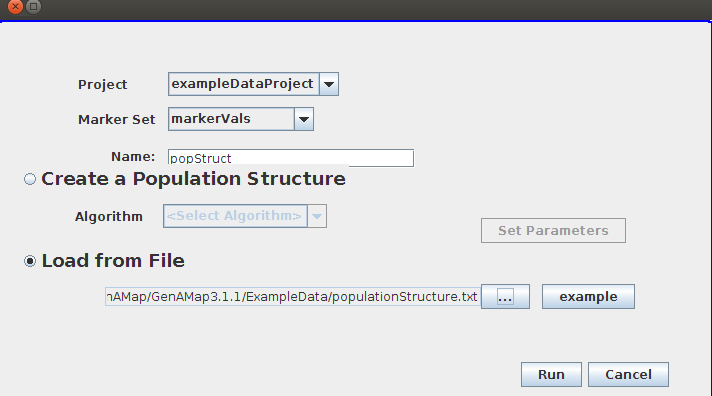
\includegraphics[width=\textwidth]{Figure9.png}
\caption{\textbf{Importing a Population Structure}}
\end{figure}

\end{document}















